\documentclass[a4paper]{llncs}

\usepackage{times,verbatim} % Please do not comment this

\usepackage[]{graphicx}
\usepackage{url}

\begin{document}

\pagestyle{empty}

\mainmatter

\title{Discovery Services Interconnection}

\titlerunning{Discovery Services Interconnection}

\author{J\'{e}r\^{o}me Le Moulec\inst{1} \and Jacques Madelaine\inst{1} \and Ivan Bedini\inst{2}}

\authorrunning{J\'{e}r\^{o}me Le Moulec et al.}

\institute{GREYC -- CNRS UMR 6072,\\
Bd Mar\'{e}chal Juin,
F-14000 Caen, France\\
\email{\{jerome.le\_moulec, jacques.madelaine\}@info.unicaen.fr}
\and
Orange Labs.\\
42, rue des Coutures,\\
F-14000 Caen, France\\
\email{ivan.bedini@orange-ftgroup.fr}}

\maketitle


\begin{abstract}
  This paper presents and discusses various solutions for the cooperation of several components
implementing Discovery Services (DS) in the EPCglobal architecture. This architecture aims to
collect and store events involving objects tagged with a Electronic Product Code (EPC) that can be
accessed using the RFID technology. Each event is stored in a repository with a standardized
interface specification: the EPC Information Services. The DS components are used by the application
layer in order to retrieve which repositories store events about a given code. If this is not a
problem for a centralized network, it is still an open question for a decentralized architecture.
Security and access controls concerns are also taken into account.
\end{abstract}

\section{Introduction}

The EPCglobal architecture aims to query events about things collected by the network. Hardware
readers acquire the so called Electronic Product Codes (EPC) from tags using the RFID technology.
Each event is stored in a repository with a standardized interface specification: the EPC
Information Services (EPCIS).

As each organization has its EPCIS, information about the supply chain can be retrieved and
processed by an application layer, if it knows which EPCIS are concerned with a given EPC code. If
this application is standardized for a centralized network with the Object Naming Service (ONS) and
the Discovery Service (DS), the problem is still open for a decentralized network using several
component for the Discovery Services~\cite{BRIDGE},~\cite{dsdesign},~\cite{tracabilityDS}.  

We present in the paper three solutions for the interconnection of the components of the Discovery
Services. The solutions are designed not to introduce to much change in the other services
specifications of the EPCglobal architecture. Another concern is in the security and access control
enforcement. Then we propose a first solution based on peer to peer technology to share information
among the components of the Discovery Services. A second solution using XML routing is presented.
Lastly, a solution giving more importance to the ONS is given. As this last solution seems more
promising to take into account security and access control, we choose to implement it in a
experimental platform we are currently deploying jointly with Orange Labs and the GREYC laboratory.
The paper is organized as follows. Section 1 recalls the EPCglobal
architecture and motivates the needs for several components in Discovery Services implementation.
The following sections present the three solutions for DS interconnexion. Finally, the conclusion
presents future works.

\section{EPCglobal}

%\subsection{What Is It?}

EPCglobal~\footnote{\url{http://www.epcglobalinc.org}} has been created with the specific purpose to
develop a universal identification system and an open architecture to provide interoperability in
complex supply chain scenarios. This universal identification system is based on assigning a unique
Electronic Product Code (EPC) included in each product (entity) by using tags. These tags ensure a
world traceability using the RFID technology. The applications of the EPCglobal network is not
restricted to classical supply chain management, but may be use, for instance, in luggage management
in airports.

\subsection{The EPCglobal Network}

The EPCglobal network is structured in layers. Figure \ref{epcglobalarchi} shows the data available
into the various levels of this architecture. Note that all the layers are completely disjoint and
communicate only with messages exchanged over the network. These messages use XML and their
structures are normalized by the EPCglobal Organization~\cite{dsconcept},~\cite{epcis}.
This section describes the different layers as they are defined by the EPCglobal Organization. 
%It presents each layer role in the EPCglobal network architecture. 

\begin{figure}[htb]
\centering
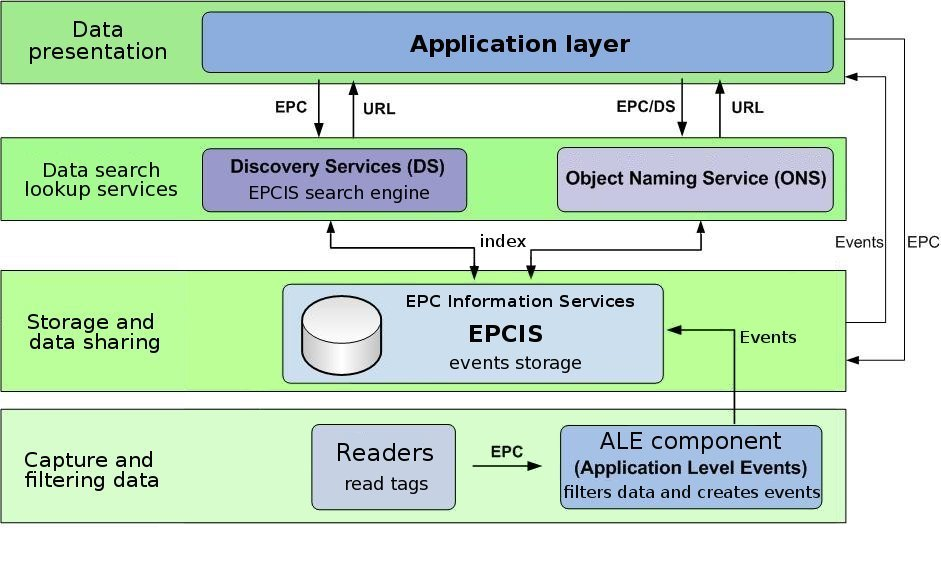
\includegraphics[width=0.7\textwidth]{img/epcglobalarchi2.jpg}
\caption{EPCGlobal Network General Architecture}
\label{epcglobalarchi}
\end{figure}

The bottom layer involves hardware that can read RFID tags. It is also
responsible with the Application Level Event component (ALE)~\cite{ale} to detect read
failures and to create events with the codes read from the tags. It is configured to add several
informations such as ``business step'', ``read point'', ``message type'',
``timestamp''\ldots{} Furthermore, it will filter the data in order to send only
once an event concerning a given code. It does
not store any data and only provide events to the upper layer. The upper layer
deals only with events formatted as valid XML entities. 

The next layer is for the storage and the data sharing. This is achieved by the EPC
Information Services component (EPCIS)~\cite{epcis}. It is made of the EPCIS repository,
designed to store received events. It has two interfaces: the EPCIS capture
interface, used to capture events sent by the lower level layer and the EPCIS
query interface, set up to retrieve the stored information.

The third layer, the lookup layer, contains the services that we want to enhance
with the proposition of this paper.  In complex scenarios where the industrial
process is not just managed by a private network and involves more than one firm,
informations are spread over multiple EPCIS servers. Therefore a lookup layer is
mandatory. The Object Naming Service (ONS)~\cite{ons} carries out the indexing
of EPCIS manufacturers and can deliver their IP address. ONS uses the Internet's
existing Domain Name System (DNS)%~\cite{DNS}
for looking up (resolving) information about an EPC. Hence, it doesn't provide
any identification or access control policy. Everyone can retrieve any entry.
The other component of this layer, the Discovery Services (DS), is the ``search
engine'' for EPC related data. They are not limited to the entities that originally
assigned an EPC code, and may return the addresses of all EPCIS containing
information about the given EPC unless it is filtered by the access control
policy. Note the Discovery Services standard is still in development~\cite{dsconcept} . 

At the top level, we find the application layer that uses the lookup services 
in order to extract the events it is interested in, and to process and present
the information.

\subsection{Standards}
As we mentioned, the EPCglobal network is not currently fully normalized. 
%Figure \ref{standards} shows the EPCglobal organization standard process. 
The standardization process allows three standard levels types for each network component: 
data standards, interface standards and standards in development.

Today we cannot call EPCglobal architecture ``Internet Of Things''. As is, the network is ready to
be used in closed networks. That means that data exchange between firms is not currently possible or
must be controlled by the firm itself giving EPCIS network access to particular users. This job
should be realized by the Discovery Services component that is still at the moment in the standard
development process.

To set up our own EPCglobal network, we decided to study some DS specification proposals in several
projects, as the one presented in~\cite{BRIDGE}.

Finally we choose the IETF organization Internet draft~\cite{dsconcept} as a start.

\subsection{A World with several Discovery Services}

DS are presented as the ``search engines'' of EPCglobal. But, if web search engines can be
independent, it is not the case for DS. Indeed, while web search engines users expect only a
representative subset of pages addresses corresponding to their request, DS users usually want
\emph{all} EPCIS addresses storing events about a given EPC. Another difference is that, unlike
search engines with web pages, DS servers cannot crawl EPCIS servers due to data access control
concerns. EPCIS servers have to publish their events to one (or more) DS server they know. This
section motivates why it is useful to have more than one DS server.

We explained previously that DS servers must fulfill two functions: index EPCIS servers and manage
the access control policy. What happens if, for a given EPC the corresponding information is spread
over multiple EPCISs referenced by more than one DS server? It is conceivable that several companies
will want to run their DS server in order to manage their own data as also argued by K\"urshner et
al.~\cite{dsdesign}. Furthermore, it will be an opportunity to develop additional
services~\footnote{To follow the metaphor with the Internet, this problem is similar to Internet
providers interconnection}. It is therefore useful to allow DS interconnection.

The four actors supply chain scenario depicted in figure \ref{scenario} will help us to motivate the
problem 
of finding DS servers addresses. It is composed of:
\begin{itemize}
\item a factory that provides manufactured products;
\item a logistic platform, third part actor who take products from the factory to the wholesaler;
\item a wholesaler that stores the products brought from the factory;
\item a retailer that sells the products to consumers.
\end{itemize}

\begin{figure}[htb]
\centering
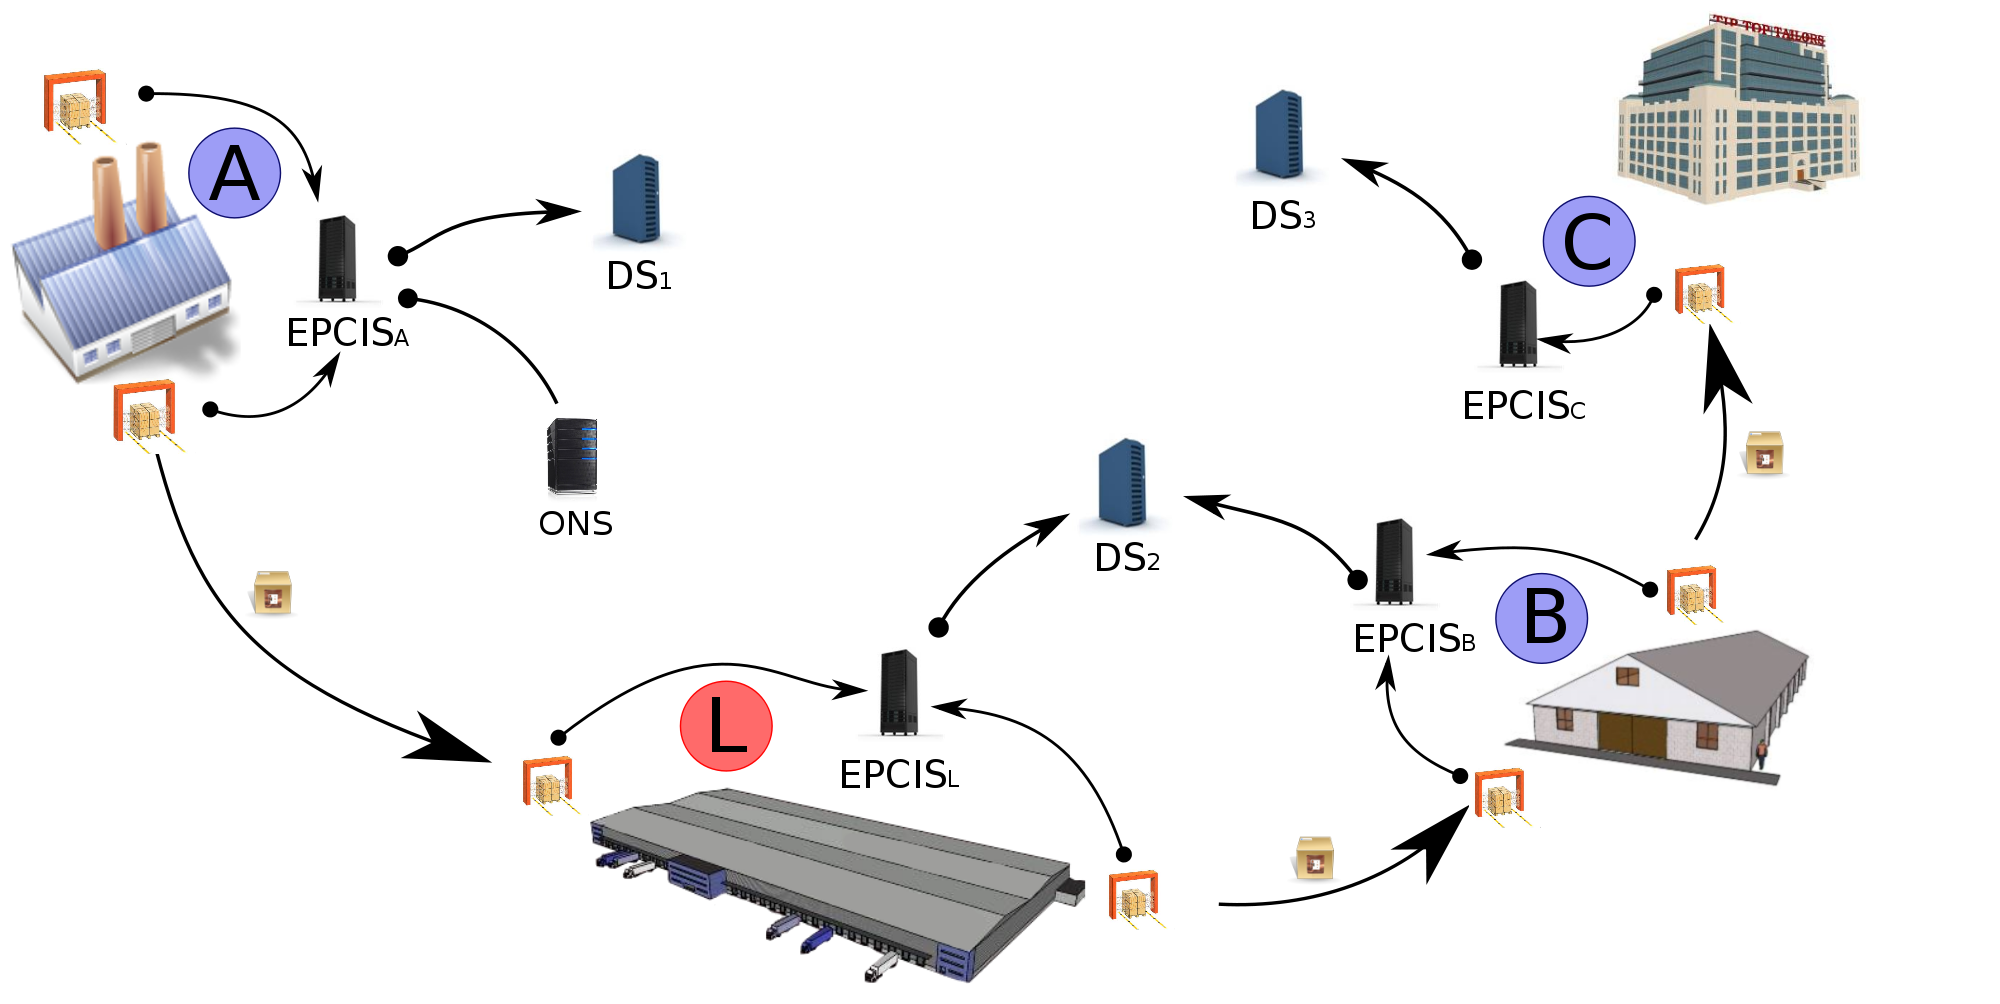
\includegraphics[width=.8\textwidth]{img/scenario2.png}
\caption{The four actors supply chain scenario.}
\label{scenario}
\end{figure}

To make our scenario more realistic, we suppose that the factory imagines that its products are
directly imported by the wholesaler whereas they are carried by our third part actor: the logistic
platform. This use case illustrates that in real conditions no actor can exactly know who are the
next ones in a business process. This test case will be useful to show that the network will be able
to find a lost product even if this information is kept by an unknown actor.

For a given EPC that passes through this supply chain, the corresponding events will be spread over
four EPCIS (A B C and L). Consequently, for this same EPC, the DS server 1 will index the EPCIS~A,
the DS2 will index EPCIS~L and EPCIS~B, and the last one, the DS server 3 will index EPCIS~C. How
every user will be able to retrieve all the information? Currently, it will have to know the three
DS servers addresses to query them one by one. We pictured out several solutions in the next
sections:

\begin{itemize}
\item share the DS-repository between all DS servers using Peer to Peer technologies;
\item dynamically chain EPCIS servers using publish/subscribe XML routing technologies;
\item give a particular role to a chosen DS server (the \emph{referent} DS) and reinforce the ONS server role.
\end{itemize}

In this paper we do not investigate the LDAP solution that is already discussed by Cantero et
al.~\cite{tracabilityDS} that seams to be a good solution for optimal response time to queries but
is poor for distributed updates.
%The following solutions use this scenario with the same EPCglobal architecture. The purpose is to
complete it with a new layer enabling DS servers communications. Any user must be able to retrieve
all information on the corresponding product by knowing one and only one well known start point (for
example an ONS address). 


\section{The Peer to Peer alternative: DS like a Peer}

We study in this section the possibility to use peer to peer facilities to allow DS servers
communication. Indeed, each DS server can keep a subset of the global index repository using a
Distributed Hash Table (DHT). Distributed Hash Tables are a class of decentralized distributed
systems that provide a lookup service similar to a hash table .Pairs are stored in the DHT, and any
participating node can efficiently retrieve the value associated with a given name. Responsibility
for maintaining the mapping between names and values is distributed among the nodes, in such a way
that a change in the set of participants causes a minimal amount of disruption. This allows DHTs to
scale to extremely large numbers of nodes and to handle continual node arrivals, departures, and
failures.

Figure \ref{P2P} shows the new architecture incorporating a Peer to Peer interconnection network. DS
servers are seen like P2P nodes according to the above DHT definition. These servers need to
implement all Peer to Peer protocols as discovery, data exchange\ldots{} It is useless to modify
neither the existing EPCglobal layers architectures nor layers communication specifications. This
solution allows to add or remove DS servers in a very simple way.

\begin{figure}[htb]
\centering
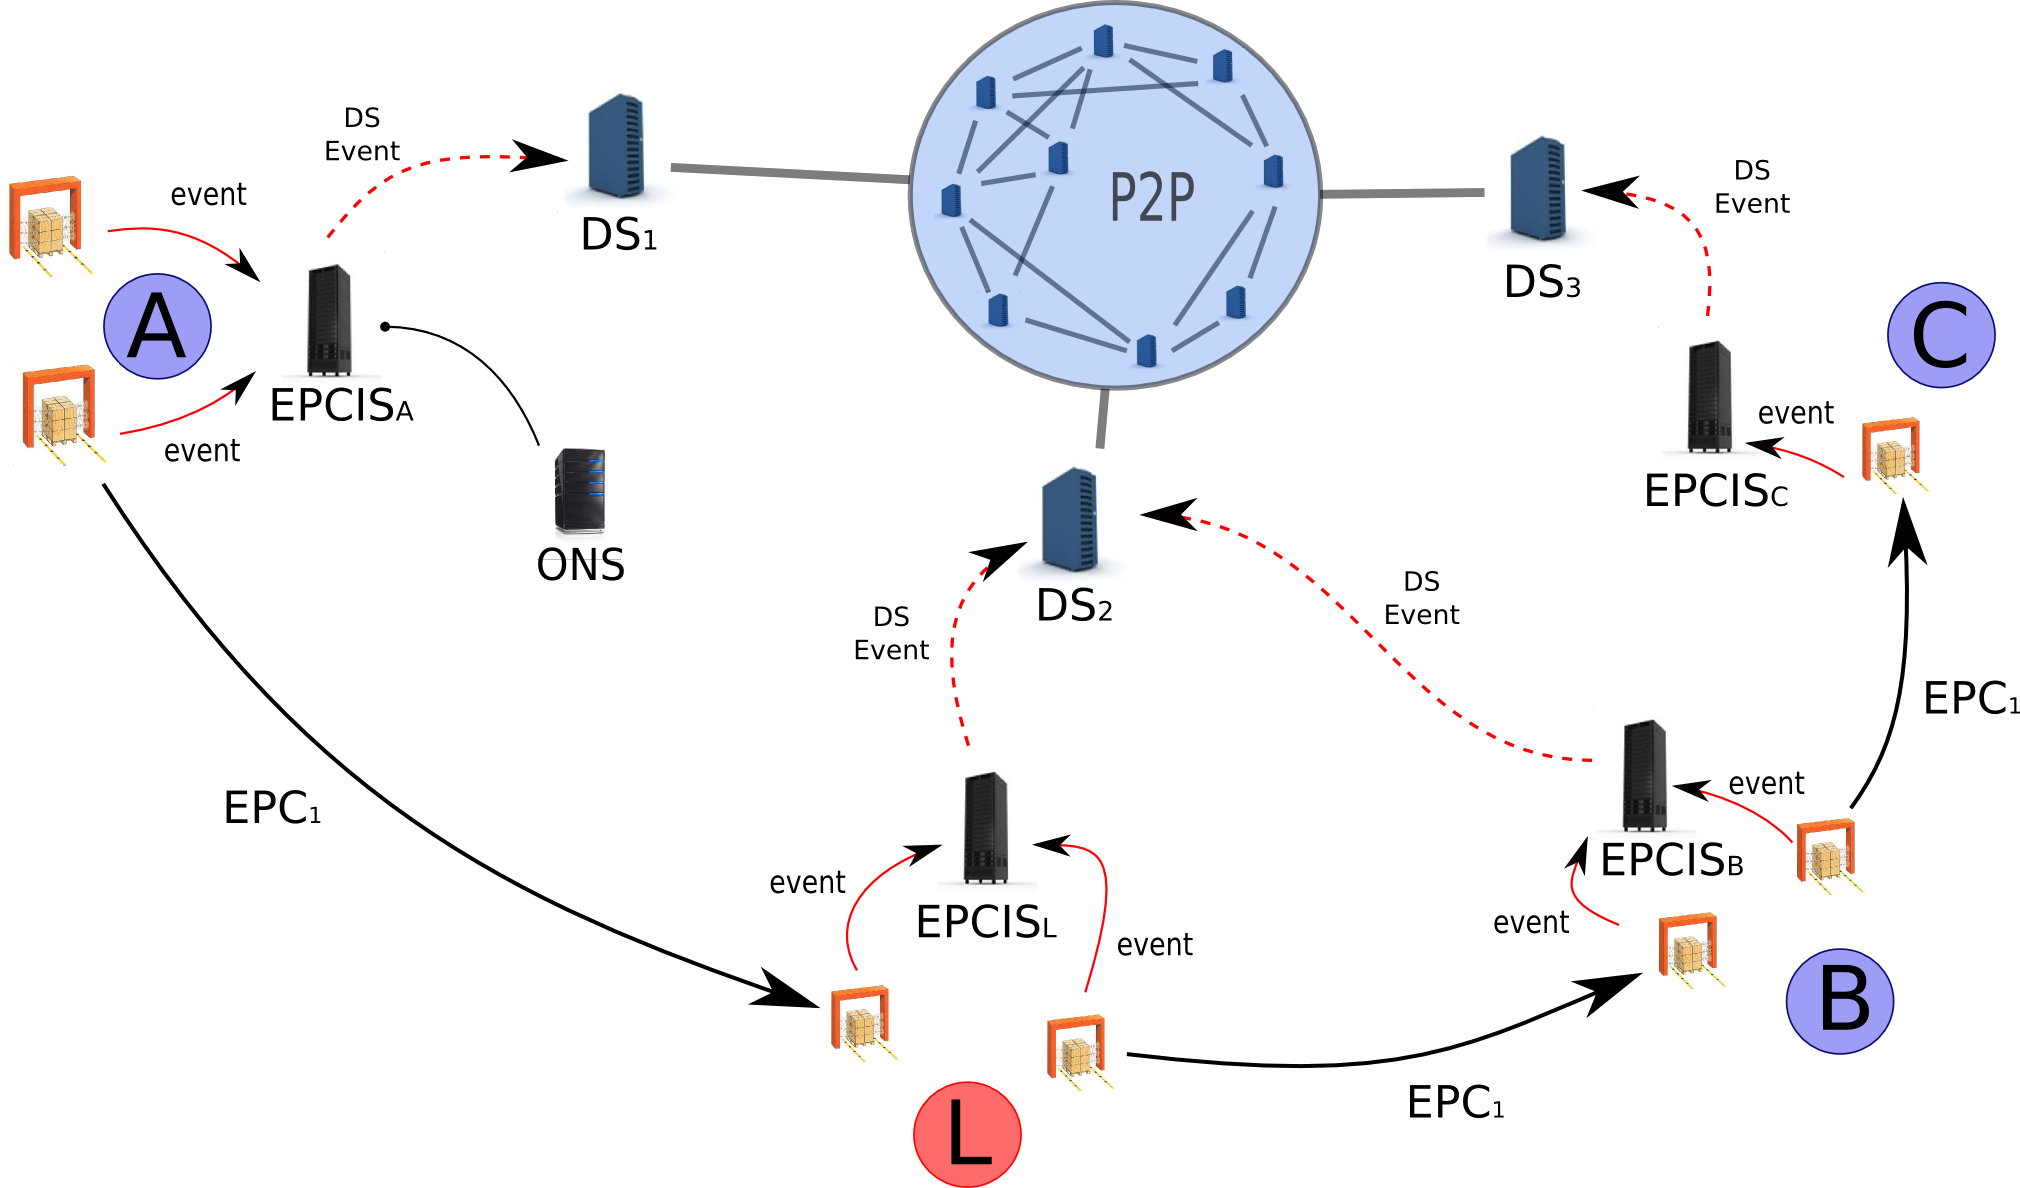
\includegraphics[width=.8\textwidth]{img/p2p.png}
\caption{Peer to Peer data sharing.}
\label{P2P}
\end{figure}

If we have a look at our example, as soon as the product leaves the factory, it is detected by the
reader. The corresponding informations (from the ALE component) are sent to EPCIS~A. This latter
saves the incoming event in its EPCIS-repository and publishes the corresponding DS event to the DS
server 1 who finally saves the incoming event in its DS-repository (its part of the DHT). Then, DS1
uses P2P protocols to inform other peers (other DS servers) that it has just add a new event in its
repository and pushed the corresponding key (the EPC). The same process happens when the object is
detected while it enters the logistic platform. But, at that time, the DS server 2 receives the DS
event from EPCIS~L and saves it in its own repository (its part of the DHT). The corresponding key
is shared using peer to peer protocols.

The user who wants to retrieve information for that object can query any DS server. They can all
retrieve this information thanks to P2P discovery and data transfer protocols.

\subsubsection{Discussion}

This solution does not affect the EPCglobal architecture. It simply allows data exchange between DS servers. It is designed to be very fast and to use standardized protocols. It provides a lot of start points because all DS servers can retrieve and manage the entire distributed index.

However, several points must be detailed. The usage of P2P has been already investigated by Huang et
al. in the distributed ePedigree architecture~\cite{epedigree} and in the BRIDGE
project~\cite{BRIDGE}. Nevertheless the former, ePedigree, provides a P2P based implementation that
does not consider security and access control aspects, focusing only on an EPCIS closed environment.
While the latter leaves security issues to the system responsibility. Still remains the problem to
manage security and access control policy. In fact the underlying P2P network is based on a publicly
shared DHT leading anybody be aware of the existence of a code in a specific EPCIS. This point deals
with data confidentiality that can be valuable even without knowing the associated event. How to be
sure that they will not be intercepted by any malicious actor? Furthermore, another limitation of a
P2P based solution arises when a node is down. The user who queries one DS server won't be able to
know that the information he retrieves is not up to date. Moreover, the discovery protocol allows
users to retrieve as much information as possible but does not insure to retrieve all of it.

The final point concerns the underlying TCP/IP network management. To manage a real P2P network, all
nodes must have public addresses or must be mapped using NAT servers. That implies to open firewalls
on many ports and it may then be hard to manage a private network security.

\section{Multi-DS for EPCIS chaining: DS like a router}

The EPCIS chaining solution seams to be the simplest way to track products. Each EPCIS knows the
next one for a given EPC. For example, the wholesaler knows that its object goes to the retailer.
The EPCIS chaining concept involves that the firm from where the objects are sent always knows where
they will go. In our scenario the factory happens to know that it make business directly with the
wholesaler whereas there is a third actor between them. In this use case, the EPCIS of the factory
cannot know the next one, the one from the logistic platform. In the same way, we suppose that the
object is lost between the wholesaler and the retailer. How to find it again? There is no way for
the wholesaler EPCIS to know the address of the next EPCIS (it ``thinks'' that it is the retailer
one but possibly not).

This proposal uses XML routing to connect DS servers. XML routing is a XML data transfer protocol.
It allows XML document to be routed in a specific network not using the receiver IP address but
simply the content of the document. XML routing is based on a publish/subscribe service that allows
subscribers to express their interest in documents containing specific keys or values or satisfying
some patterns.

\begin{figure}[htb]
\center
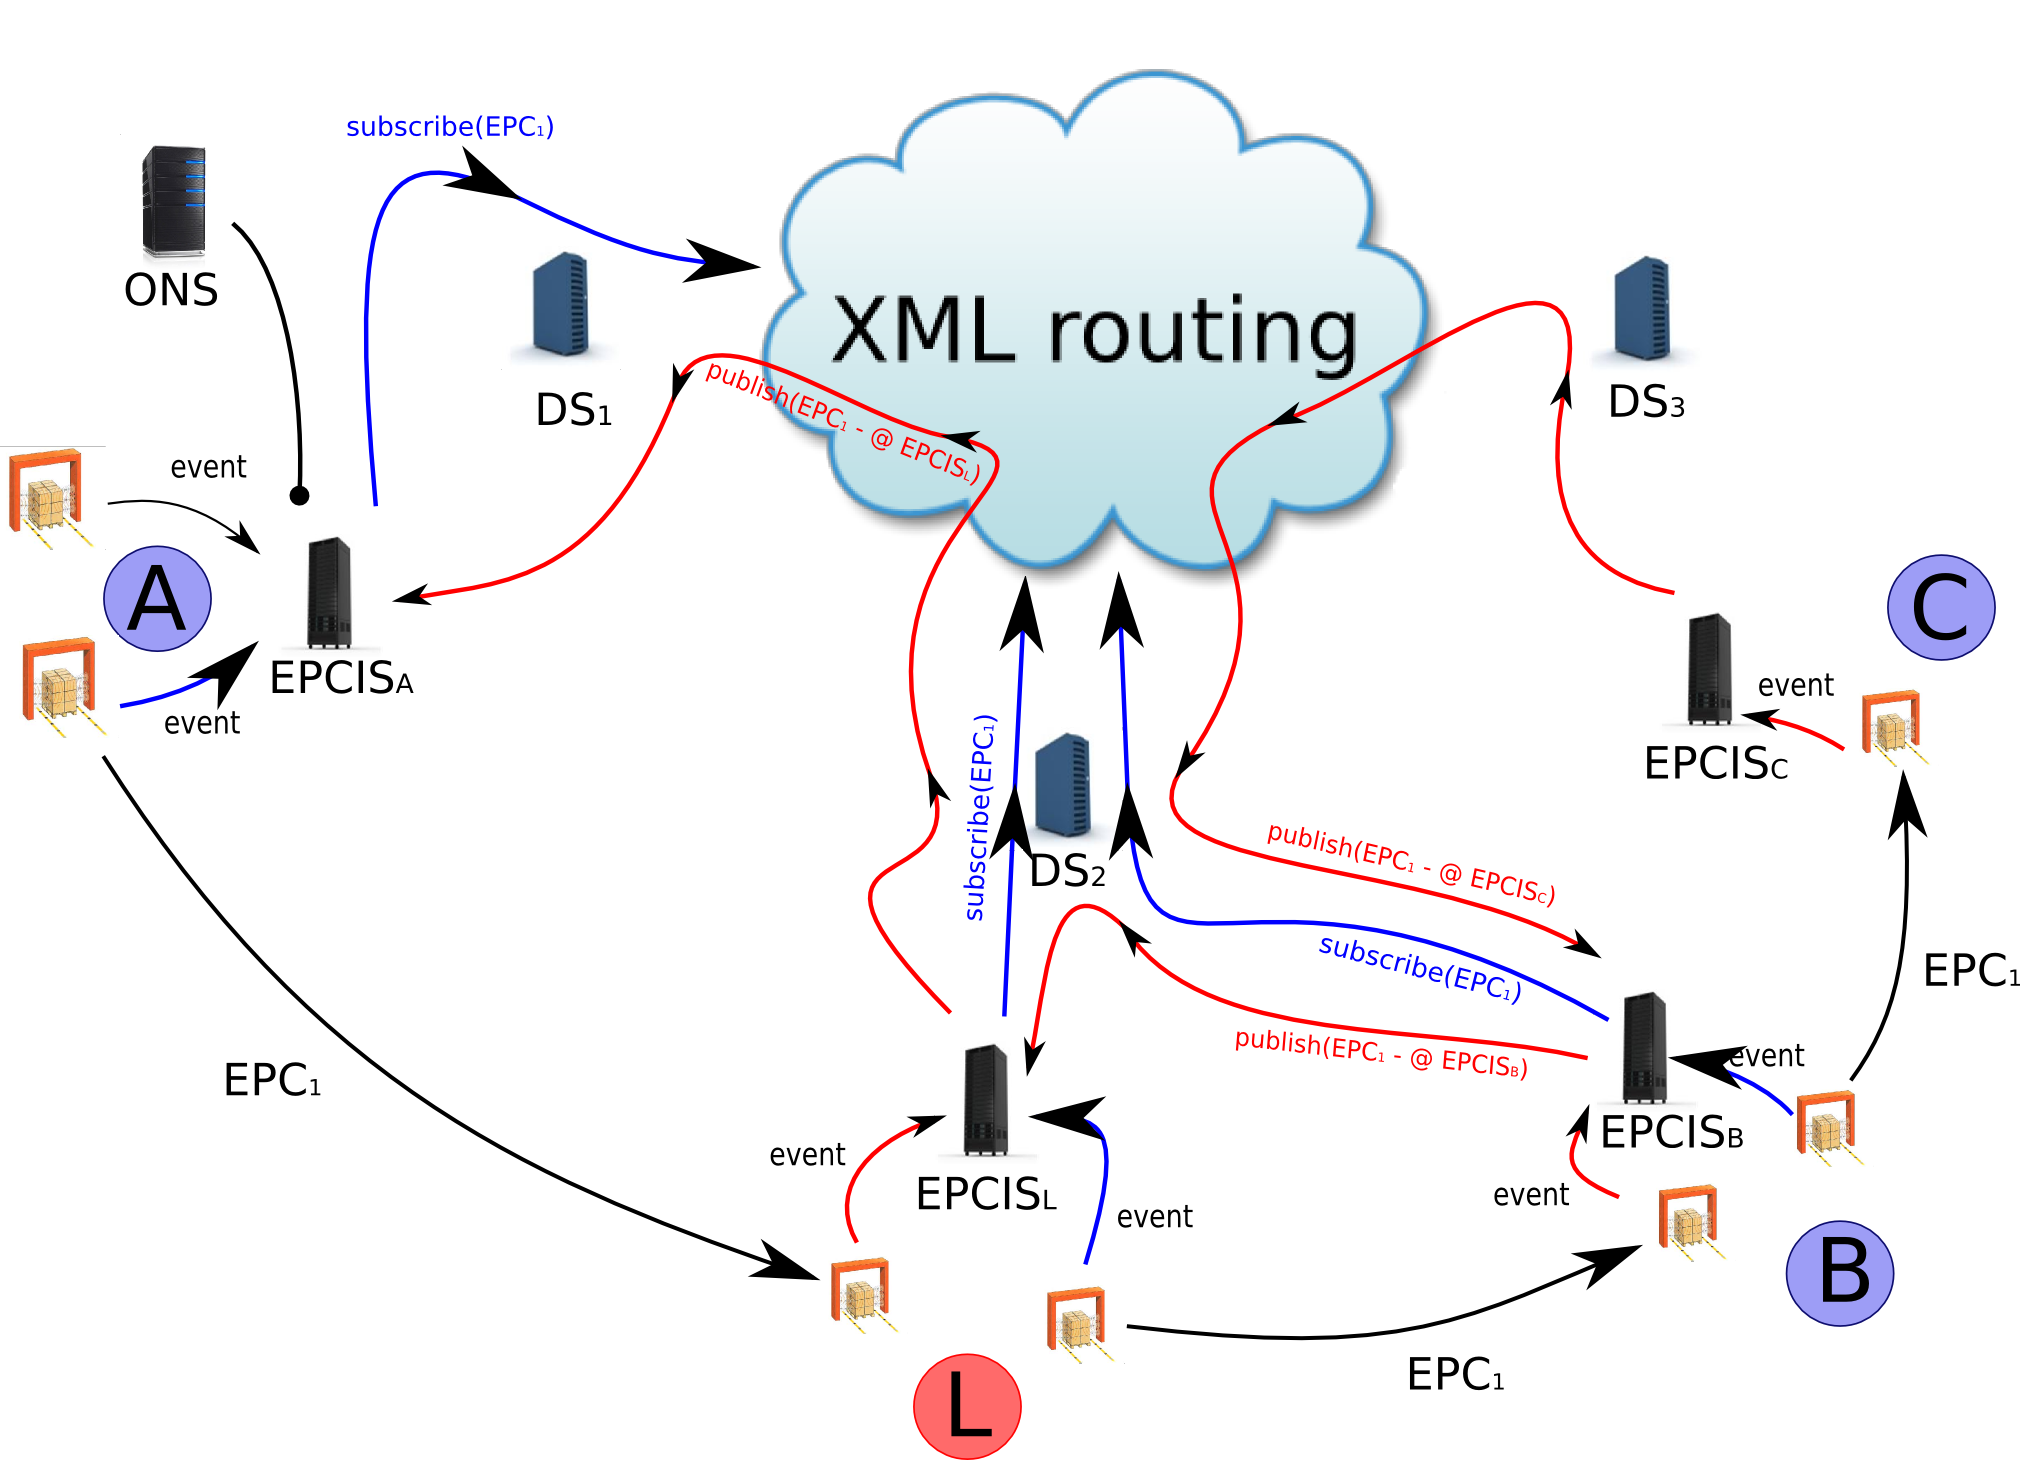
\includegraphics[width=.9\textwidth]{img/xmlrouting.png}
\caption{Multi-DS for EPCIS chaining.}
\label{epcischaining}
\end{figure}

The DS servers allow EPCISs to subscribe to the XML routing network for a given EPC. For example,
the factory creates the product \texttt{epc1}. When the object leaves the firm, the EPCIS subscribes
to the XML routing network using its DS server for XML messages containing the \texttt{epc1} value.
When the object arrives at the logistic platform, the EPCIS~L publishes an XML message containing
the \texttt{epc1} and its service address to the XML routing network using DS2. As EPCIS~A is
interested in the product type of \texttt{epc1}, it has subscribed to that XML message type, so it
receives it and saves the correspondence between the address contained in the document and the
\texttt{epc1}. In this way, each EPCIS ever knows what is the next EPCIS address in the chain for
any EPC code it is interested in. We have added here XML routers capabilities to the DS servers.

\subsubsection{Discussion}

This solution presents two main weak points.
%\begin{enumerate}
%\item
The first one is a consequence that XML routing does not support any acknowledgment. When DS2
publishes the XML document in the network it cannot know if somebody is listening and likewise if
somebody is receiving it. That may introduce lacks or errors in the EPCIS dynamic chaining process.
Let's suppose that DS1 is out of order when the XML document is sent, then it does not receive it.
When the object arrives at the wholesaler, the corresponding EPCIS (EPCIS~B) publishes a new XML
document using DS2. This message is routed to EPCIS~L but also to EPCIS~A because DS1 is now up. As
a result, EPCIS~A ``thinks'' that the next link is through EPCIS~B, but it is  absolutely not the
case.%\item 

The second problem is due to the chaining itself. We suppose now that the dynamic chaining process
was successfully realized. The user who now wants to track information about \texttt{epc1} will
query the first EPCIS of the chain (EPCIS~A).This one returns the information it kept and the
EPCIS~L address. The user queries now the second EPCIS but this latter one is down. There's no way
to retrieve all other information, as the chain is broken!
%\end{enumerate}

This solution use a real interesting concept but remains too sensitive to server failures. It is
absolutely not robust enough. Furthermore, it allows mistakes not admissible for such a network. It
also raises some other questions relative to the XML routing technology. When will one server stop
to listen to this XML document type if nothing is received? Indeed, if the product is lost and will
not be read again by any reader connected within EPCglobal network, how to dynamically warn the
listening DS servers that they can terminate their subscription? We supposed that each EPCIS server
subscribes to the network when a product has left its firm and publishes a XML document when a
product arrives. How to detect that a product leaves or arrives in a firm? Using business step? Will
all firms use the same notation for these events? There are too many questions that makes this
solution finally too complicated.


\section{Multi-DS and ONS: DSs indexing DSs}

Let's recall that the ONS system is designed to reference the EPCIS where a particular EPC product
type appeared for the first time (in our example, from the factory). Our third proposal consists to
enhance the ONS system role: it does not only reference the EPCIS, but also its connected DS
servers.

Companies, that can assign EPCs, declare their EPCIS address in front of the object type (EPC
without serial number) in the ONS system configuration. As is, they also declare there DS server
address. Then, when any DS server receives an event, it can extract the EPC out of it and query the
ONS system to retrieve the corresponding DS address. If that address is not its own address, it
sends a new DS event to this address that we call the \emph{referent} DS server. In this new
context, for a given EPC, the referent DS indexes also the other DS servers that reference EPCIS
dealing with that same code.

\begin{figure}[htb]
\center
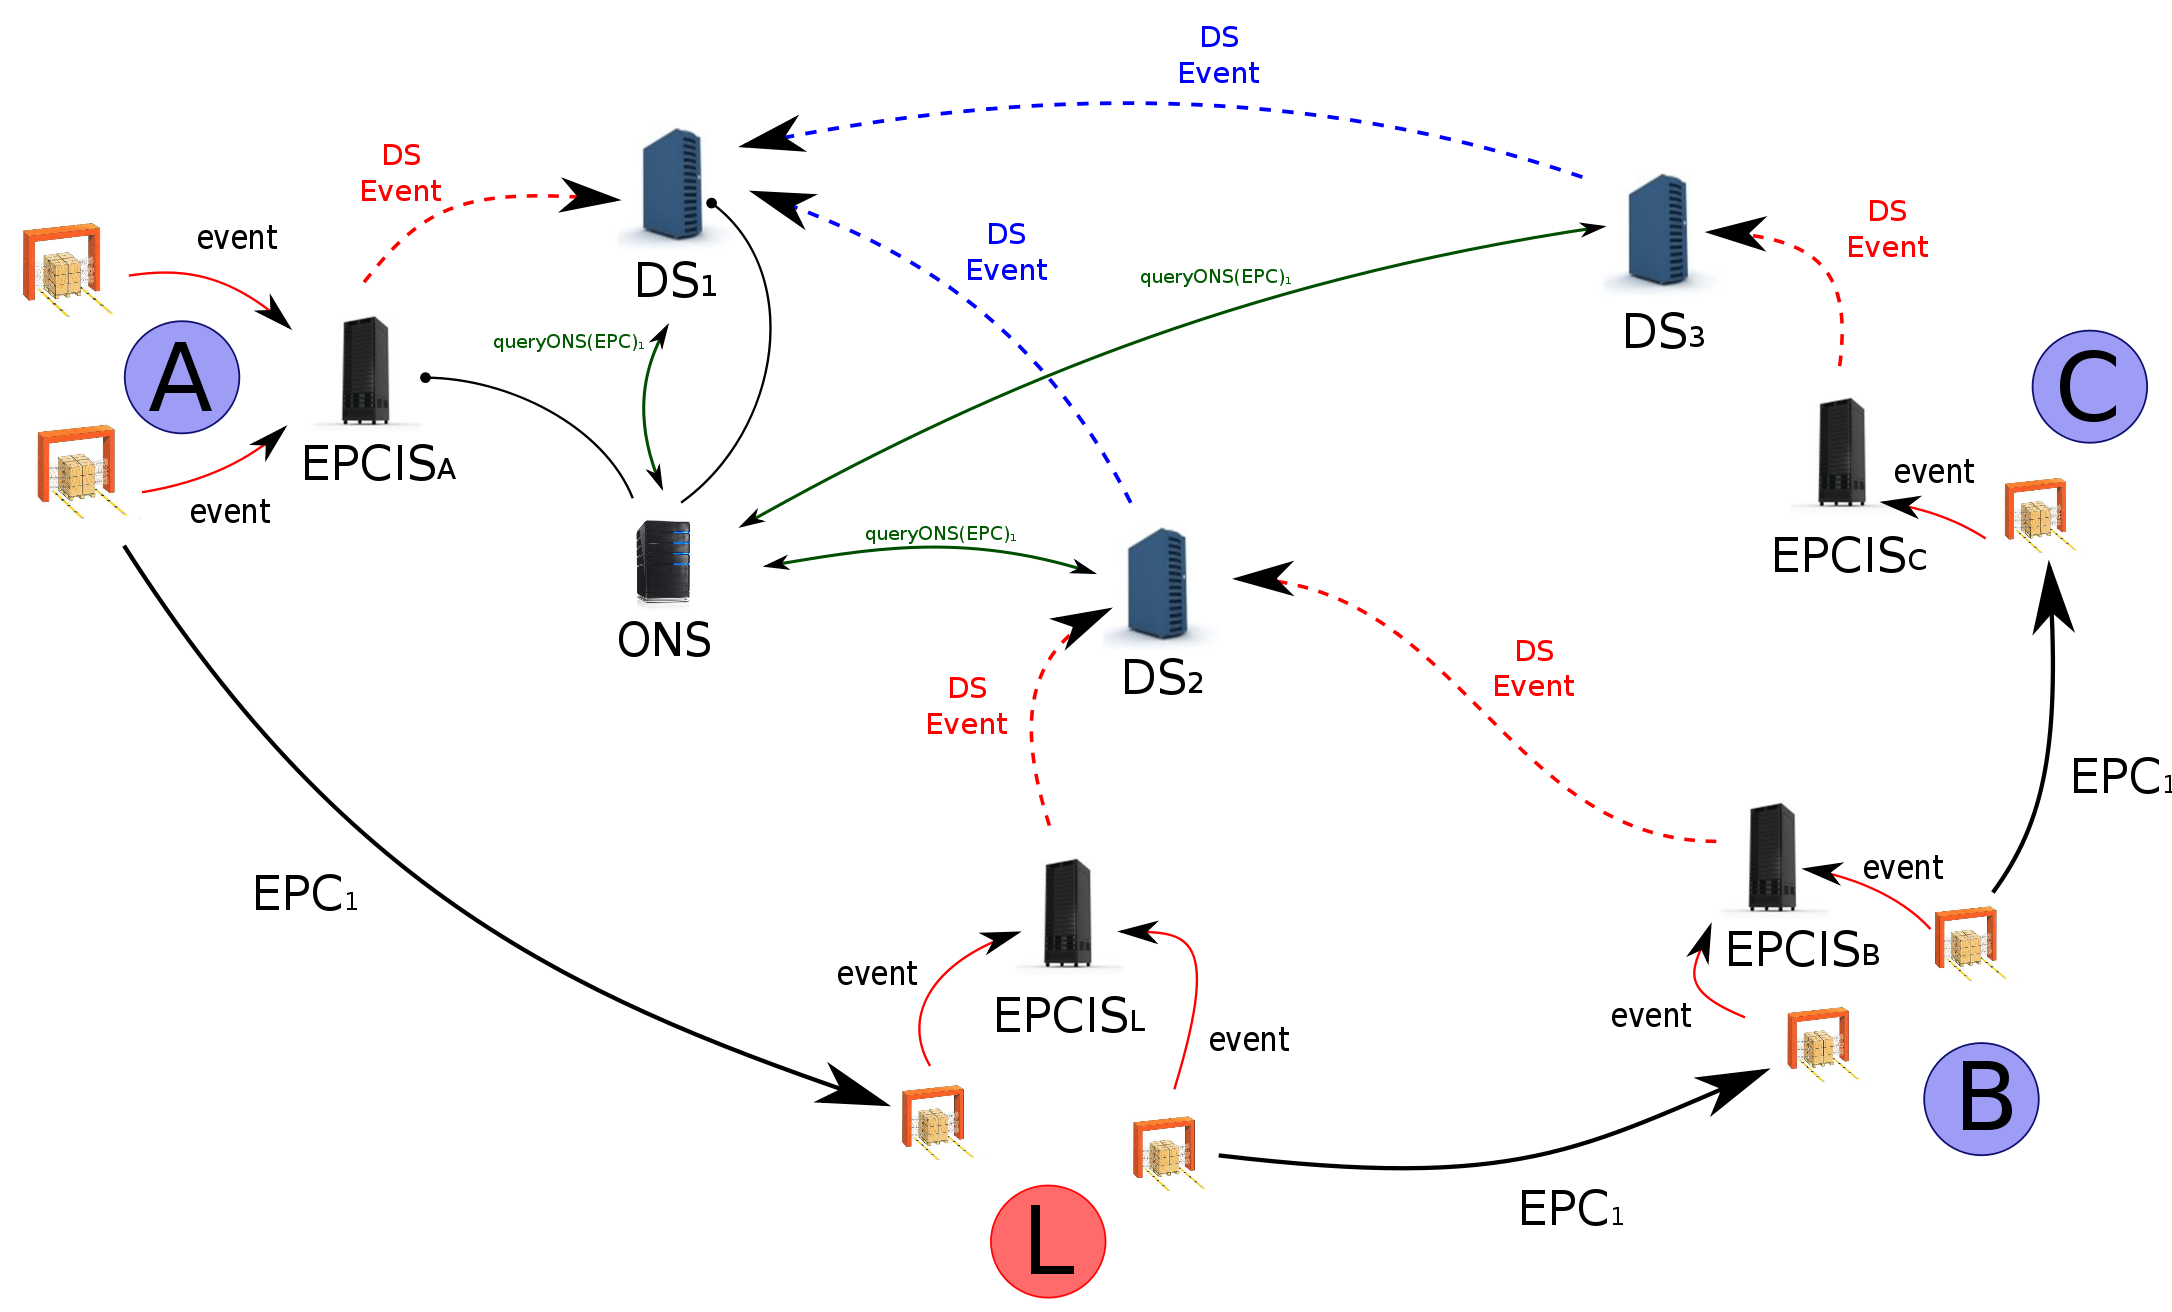
\includegraphics[width=.8\textwidth]{img/platform-3.png}
\caption{Multi-DS and ONS.}
\label{dsons}
\end{figure}

Consequently, in order to retrieve information about a given product, the application layer can
query the ONS system to find the referent DS address. Then, it queries the corresponding server to
retrieve indexed EPCISs and DSs. It does the same process again whenever new DS addresses are found
and retrieves all other EPCIS addresses. The whole information is then reachable.

Each DS keeps its own access control policy. It means that each user must identify itself before
querying anything to a DS. In our use case, a user who wants to track the product must create an
account on the three DS servers. Each company must specify, in its own DS account, that it has
agreed to share information with that user. Otherwise, if, by example, the logistic platform company
does not specify (in the DS server 2) that it has agreed to share events, no user will be able to
retrieve the EPCIS~L address. 

If we have a look at our four actors supply chain scenario, let's see what happens when the product
arrives in the logistic platform using this solution.

The product is first detected by the reader when it enters the platform. The corresponding ALE
component generates an event and publishes it in the EPCIS~L. The EPCIS~L stores the event in its
own database (EPCIS-repository) and publishes a DS event to the DS server 2 to tell that it has
information about the corresponding EPC. DS2 then stores the DS event in its own database and
queries the ONS system for the referent DS address corresponding to that code. The answer is the
address of the DS server 1. DS2 sends a new DS event to DS1. Finally, DS1 stores the new DS event in
its own database.

We suppose that our user has already created accounts on the different DS servers and all companies
agreed to share information with him. He queries first the ONS system that answers with the DS
server 1 address. Then, when queried, the DS1 answers three addresses: those of EPCIS~A, DS1 and
DS2. He will now query in turn the two new DS servers that respectively answer the addresses of the
three EPCIS L, B and C.

\subsubsection{Discussion}

This solution reinforces the ONS system role. It is now the first start point to query the network.
Contrary to the two first proposals, this architecture does not fall in case of server failures.
Every component can keep a ``to publish event'' list and periodically send it until the other server
answers that the transaction succeeded. The other strength of this alternative is that each DS is
the master for its information and is able to manage its own access control policy.

%\subsection{Security}

\section{Conclusion}

This paper has presented three different solutions for the interconnection of distributed Discovery
Services servers. Regarding confidentiality and reliability concerns, we prefer the third solution:
DSs indexing DSs. Nevertheless, some points remains to study deeply.  What happens in a real use
case with a huge number of events to publish? How will the network scale with the number of records?
Will the DS-repository not grow to fast?

We plan to answer to these questions thanks to the experimental platform we currently develop. It
implements a EPCglobal platform gathering several EPCISs and DSs interconnected using the last
solution. Several realistic scenarios are experimented in order to show the feasibility of this
solution.
The next step will be the enforcement of access control policies.

%\section{IOTA Platform}
%The IOTA (Internet Of Things Architecture) platform is a nine actors EPCglobal network. Figure \ref{scenario1} represent the physical network. It is composed by three material factories, two manufactures that put materials together to make a new product, three wholesalers and one retailer.
%\begin{figure}[htb]
%\center
%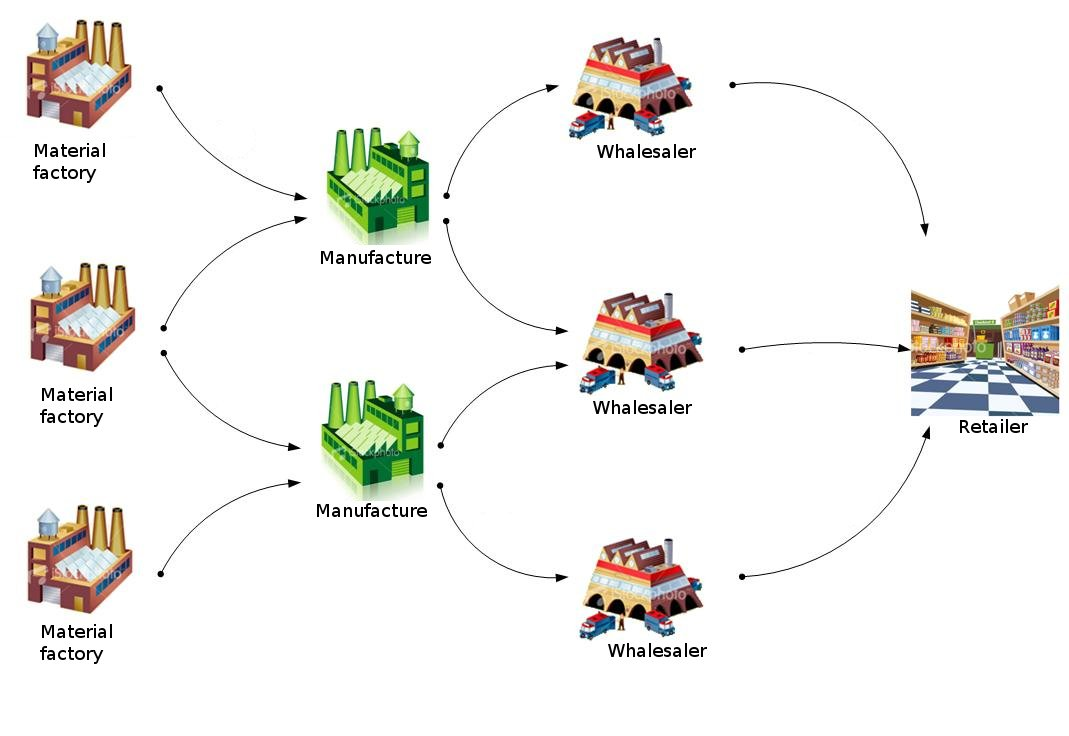
\includegraphics[width=0.8\textwidth]{img/Scenario1_2.jpg}
%\caption{IOTA physical supply chain.}
%\label{scenario1}
%\end{figure}


%\subsection{Deployment}
%The platform gathers nine EPCIS servers, three DS servers and is connected to the real ONS system. The platform is deployed over three companies. Each of them keeps a part of the platform. The University of Caen (France) holds three EPCISs and one DS server. Orange RD Caen (France) holds four EPCISs, one DS and two local ONS roots' connected. Finally, the Certic (resource platform in computer sciences) in Caen (France) holds two EPCISs and one DS server. We underline that it is useless to use three DS servers for such a small network but this platform is primarily designed to test the DS servers interoperability. Figure \ref{iota} present the platform deploiment. 
%\begin{figure}[htb]
%\center
%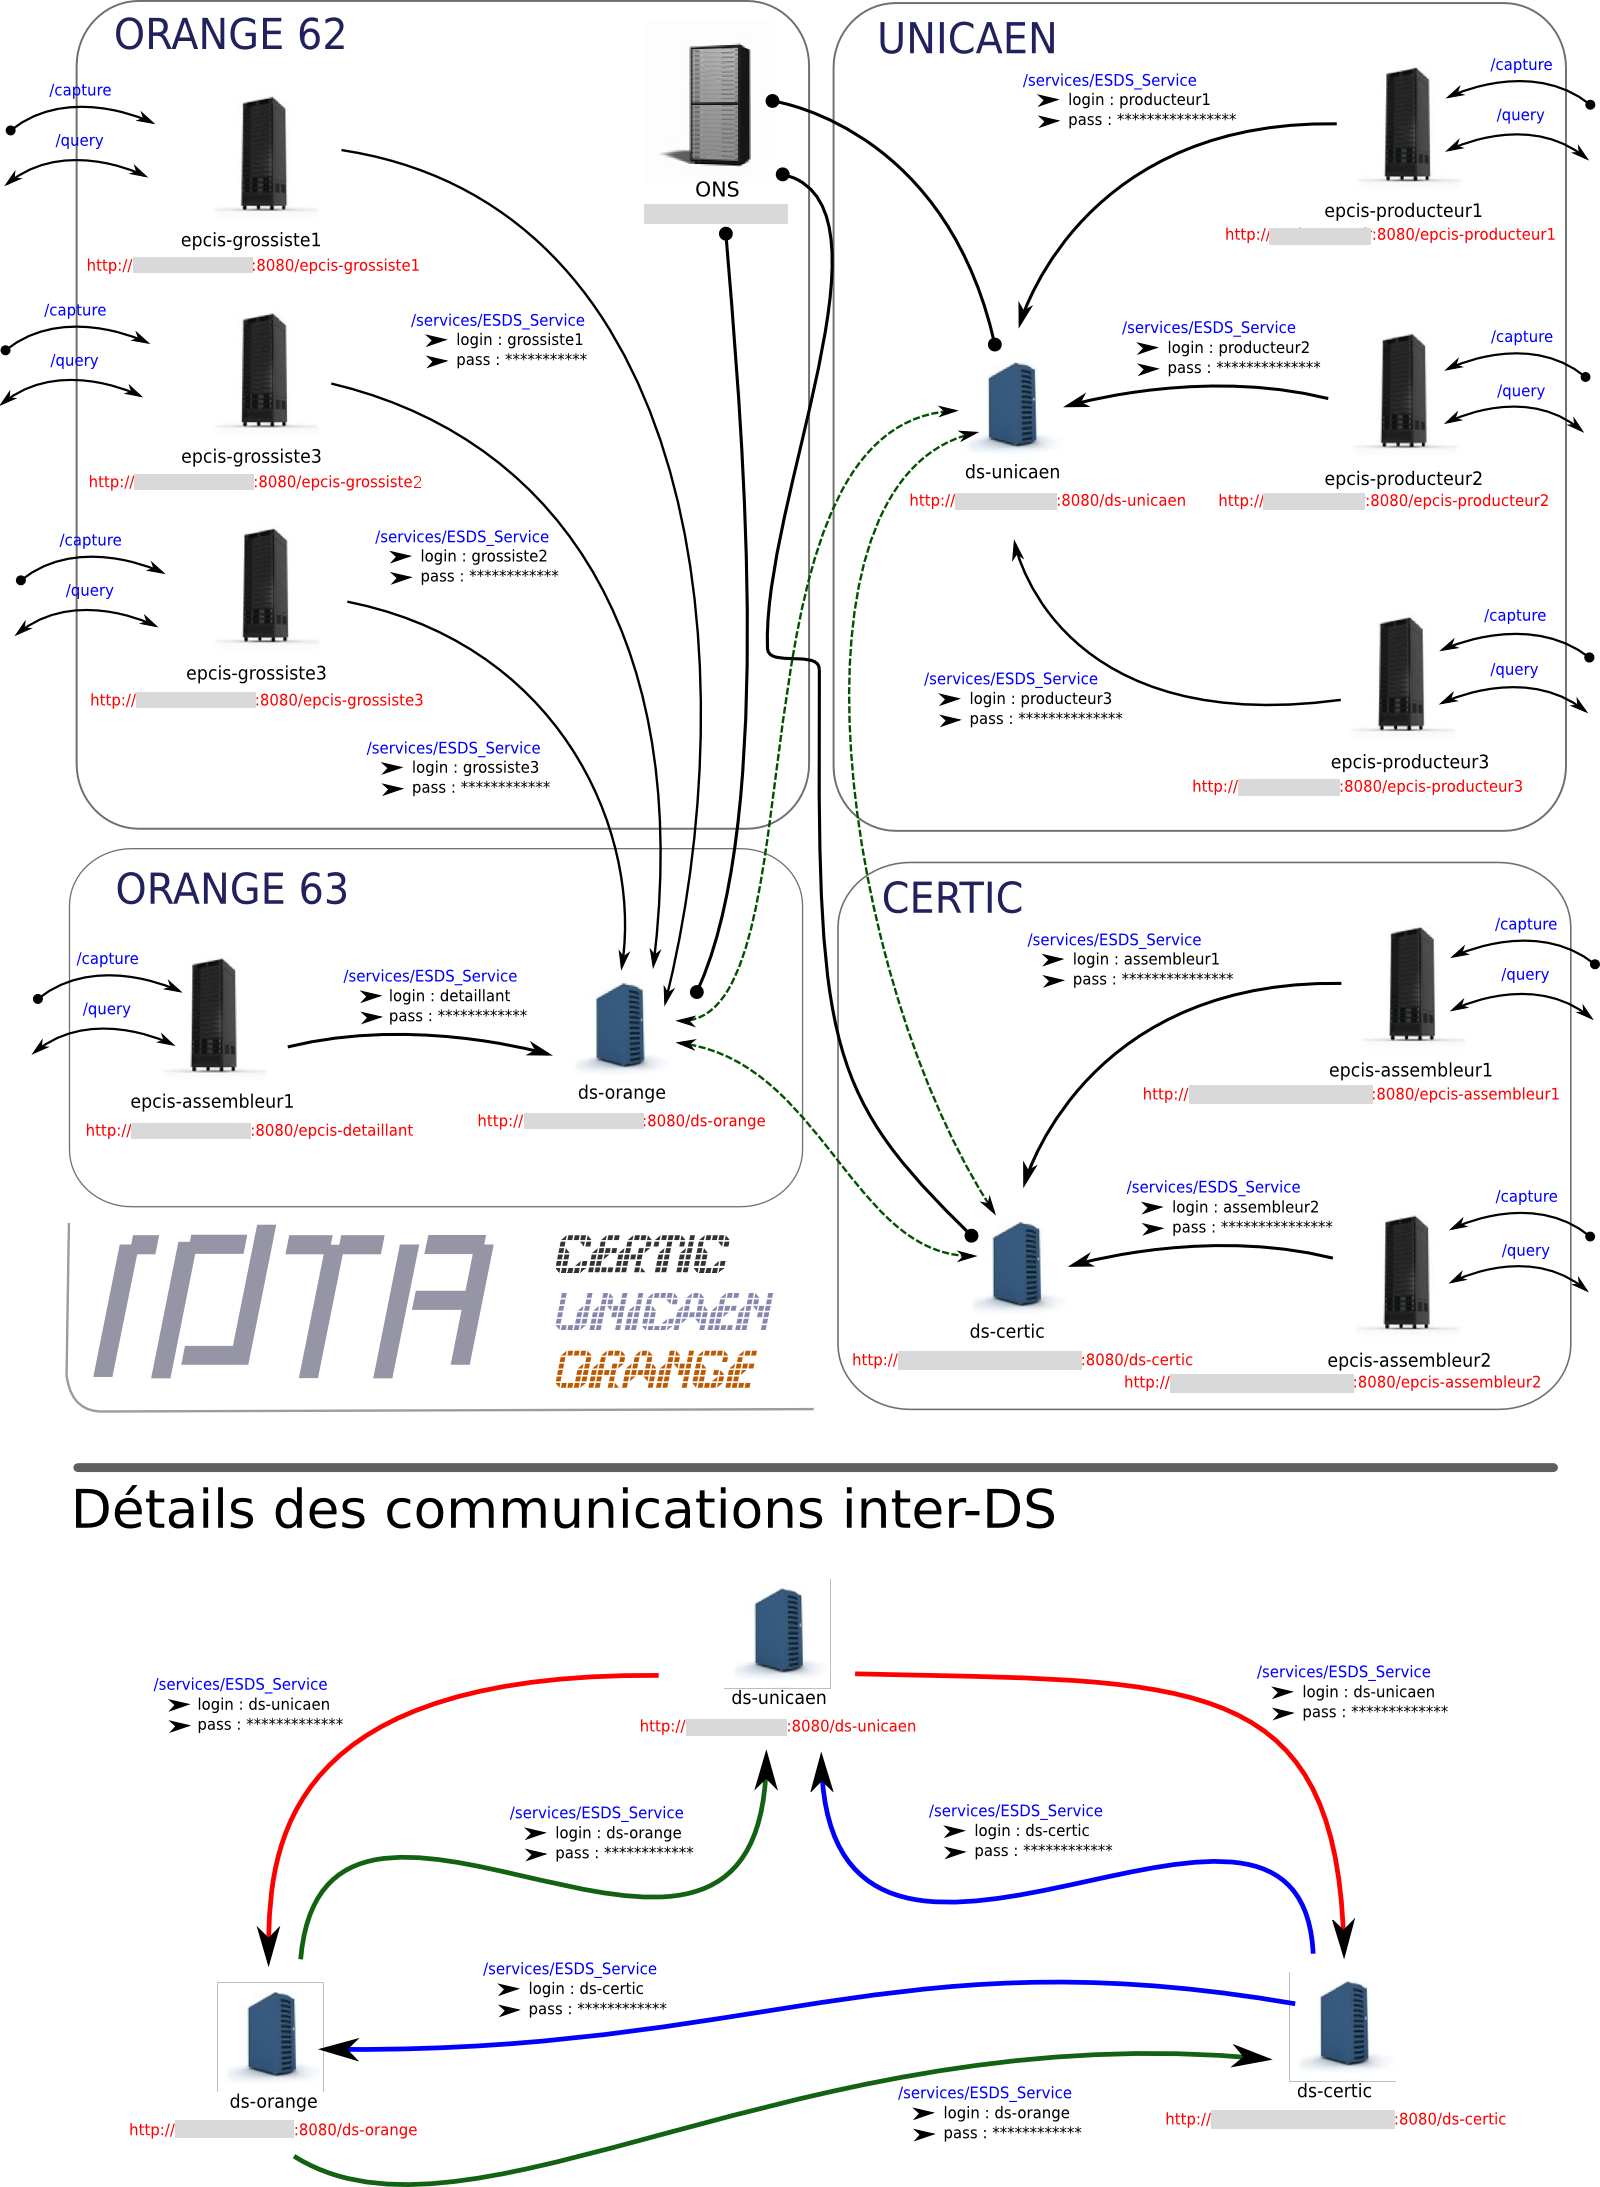
\includegraphics[width=0.8\textwidth]{img/IOTA.png}
%\caption{IOTA platform deployment.}
%\label{iota}
%\end{figure}
%The solution used to install our three DS interoperability is the third one, ``Multi-DS and ONS''. It seems to be the better one for several reasons, notably sturdiness. The platform allows four companies to create EPCs and to assign them on products. Those firms are the three material factories and the two manufacturers. Each one must reference their EPCIS and DS addresses:
%\begin{itemize}
%\item DS1 is the referent DS for the materials manufactured in the three material factories;
%\item DS2 is the referent DS for the products made in the two manufactures.
%\end{itemize}
%We notice that the lower layer is not specified. Indeed, readers and ALE components are all simulated by an underlying petri network. It allows use to grow all component databases using real scenarios without querying real firms to invest in readers. 
%The goal of creating such a network is to try to answer the previous questions concerning the solution sturdiness and to test it in real conditions (with lots of events).

\bibliographystyle{plain}
\bibliography{bib}

\end{document} 
